% !TeX program = pdflatex
% Raices que siempre estan ahi -- las raices virtuales de un polinomio real en Lean 4.
% Version en espanol de virtual-roots-lean.tex. Mismas figuras tikz.
% Build: pdflatex virtual-roots-lean-es.tex (dos veces, por refs)
% Verificado contra la fuente Lean 2026-06-17 (lake env lean VirtualRoots.lean y
% VirtualRootsCount.lean, exit 0; #print axioms sobre vroots_interlacing y
% card_vroots_Ioc_eq_fourierVar -> propext, Classical.choice, Quot.sound). Toolchain godsil v4.30.

\documentclass[11pt]{article}
\usepackage[T1]{fontenc}
\usepackage[utf8]{inputenc}
\usepackage{lmodern}
\usepackage{amsmath,amssymb,amsthm,booktabs,graphicx,hyperref}
\usepackage{xurl}
\usepackage[table]{xcolor}
\definecolor{ggteal}{HTML}{1B6F8C}
\definecolor{ggband}{HTML}{DCE7EB}
\definecolor{ggamber}{HTML}{E08A1E}
\definecolor{ggplum}{HTML}{7B4B94}
\usepackage[margin=1in]{geometry}
\usepackage{microtype}
\usepackage{float}
\usepackage[most]{tcolorbox}
\usepackage{tikz}
\usetikzlibrary{arrows.meta,positioning}
\setlength{\emergencystretch}{2em}
\newtheorem{theorem}{Teorema}
\newtheorem{lemma}{Lema}
\newtheorem{proposition}{Proposici\'on}
\newtheorem{remark}{Observaci\'on}
\newcommand{\lean}[1]{\texttt{#1}}
\newcommand{\R}{\mathbb{R}}
\newcommand{\V}{\mathrm{V}}
\newcommand{\Rd}{\mathcal{R}}
\hypersetup{colorlinks=true,linkcolor=ggteal,citecolor=ggteal,urlcolor=ggteal}
\newtcbox{\keybox}{on line,boxrule=0.9pt,colframe=ggteal,colback=ggband!40,
  arc=3pt,left=8pt,right=8pt,top=5pt,bottom=5pt}
\newcommand{\keyeq}[1]{\begin{center}\keybox{$\displaystyle #1$}\end{center}}
\newtcolorbox{recipebox}[1]{colframe=ggamber,colback=ggamber!8,arc=3pt,boxrule=0.8pt,
  title=\textbf{#1},coltitle=white,colbacktitle=ggamber}

\title{\bf Ra\'ices que siempre est\'an ah\'i\\[4pt]
  \large\normalfont Las ra\'ices virtuales de un polinomio real, verificadas por m\'aquina en Lean~4}
\author{Carles Mar\'in\thanks{Formalizado con la asistencia de un sistema de IA (Claude, Anthropic);
la matem\'atica es cl\'asica, y toda afirmaci\'on, delimitaci\'on de alcance y limitaci\'on es
responsabilidad del autor. La frontera de la contribuci\'on---en particular lo que \emph{a\'un no}
est\'a formalizado---se expone sin adornos en la Secci\'on~\ref{sec:boundary}, y es el n\'ucleo de
Lean, no el asistente, quien certifica las pruebas.}\\[3pt]
  \normalsize Investigador independiente\\
  \normalsize \texttt{karlesmarin@gmail.com}}
\date{Junio de 2026}

\begin{document}
\maketitle

\begin{abstract}
Un polinomio real de grado $d$ puede tener menos de $d$ ra\'ices reales, pero siempre tiene
exactamente $d$ \emph{ra\'ices virtuales}: sustitutos continuos y semialgebraicos
$\rho_{d,1}(p)\le\cdots\le\rho_{d,d}(p)$ que coinciden con las ra\'ices reales cuando estas existen y,
si no, se sit\'uan donde el polinomio m\'as se acerca a anularse. Las introdujeron Gonz\'alez-Vega,
Lombardi y Mah\'e~\cite{glm} y son el portador natural del recuento de Budan--Fourier~\cite{coste}.
Reporto una formalizaci\'on completa y \lean{sorry}-free en Lean~4 sobre Mathlib de su \emph{teor\'ia
estructural}: la construcci\'on recursiva mediante un operador de elecci\'on $\Rd_d$ que minimiza
$|p|$ en cada intervalo donde $p'$ mantiene signo constante; el recuento fundamental, que hay
exactamente $d$ (\lean{vroots\_length}); que salen ordenadas y dentro del intervalo de encuadre
(\lean{vroots\_isChain}, \lean{vroots\_subset\_Icc}); que $\Rd_d$ devuelve una ra\'iz real donde $p$
tiene una (\lean{R\_eval\_eq\_zero\_of\_le\_zero\_le}); y el \emph{entrelazado de Rolle}
\[
  \rho_{d,r}(p)\ \le\ \rho_{d-1,r}(p')\ \le\ \rho_{d,r+1}(p),
\]
que dice que cada ra\'iz virtual de $p'$ queda encajada entre dos ra\'ices virtuales consecutivas de
$p$ (\lean{vroots\_interlacing}). Sobre esa estructura pruebo despu\'es el recuento exacto de
Budan--Fourier mismo: el n\'umero de ra\'ices virtuales en $(a,b]$ iguala la ca\'ida de variaciones de
signo $\V(a)-\V(b)$ de la torre de derivadas (\lean{card\_vroots\_Ioc\_eq\_fourierVar},
Secci\'on~\ref{sec:count})---la igualdad que el teorema cl\'asico de Budan--Fourier solo acota para el
recuento tembloroso de ra\'ices \emph{reales}. Esto funde la construcci\'on de aqu\'i con una segunda,
recursiva de forma independiente, el recuento de signos \lean{fourierVar} de la formalizaci\'on
compa\~nera de Budan--Fourier~\cite{bflean}. Hasta donde s\'e---a partir de b\'usquedas en junio~2026
de Mathlib, la biblioteca \lean{mathcomp-real-closed} de Coq, el AFP de Isabelle y HOL~Light
(Secci\'on~\ref{sec:boundary})---ni las ra\'ices virtuales ni este recuento exacto a trav\'es de ellas
se hab\'ian formalizado en ning\'un asistente de pruebas; este es su primer desarrollo. Todo teorema
depende solo de los tres axiomas est\'andar \lean{propext}, \lean{Classical.choice}, \lean{Quot.sound}.
\end{abstract}

\medskip
\medskip
{\sloppy\noindent\emph{Lo que encontrar\'as aqu\'i.} Una visita guiada breve, construida como una cadena
de preguntas, una por secci\'on (Figura~\ref{fig:readermap}): \emph{cu\'antas} ra\'ices tiene de verdad
un polinomio, una vez que el recuento deja de temblar (\S\ref{sec:q1}); \emph{c\'omo} construir las $d$
mediante un operador de elecci\'on $\Rd_d$ (\S\ref{sec:q2}); \emph{por qu\'e} esa construcci\'on se
resiste a hacerse formal (\S\ref{sec:q3}); \emph{c\'omo} se entrelazan, a la manera de Rolle
(\S\ref{sec:q4}); y \emph{cu\'antas} caen en un intervalo---el recuento exacto de Budan--Fourier
(\S\ref{sec:count}). El desarrollo son dos ficheros Lean, \lean{VirtualRoots.lean} (la estructura) y
\lean{VirtualRootsCount.lean} (el recuento); los lemas que soportan el peso est\'an en la
Secci\'on~\ref{sec:blocks}, los l\'imites honestos en la Secci\'on~\ref{sec:boundary}. Si solo lees dos
cosas, lee el entrelazado (Teorema~\ref{thm:interlace}) y el recuento (Teorema~\ref{thm:count}).\par}

\begin{figure}[htbp]
\centering
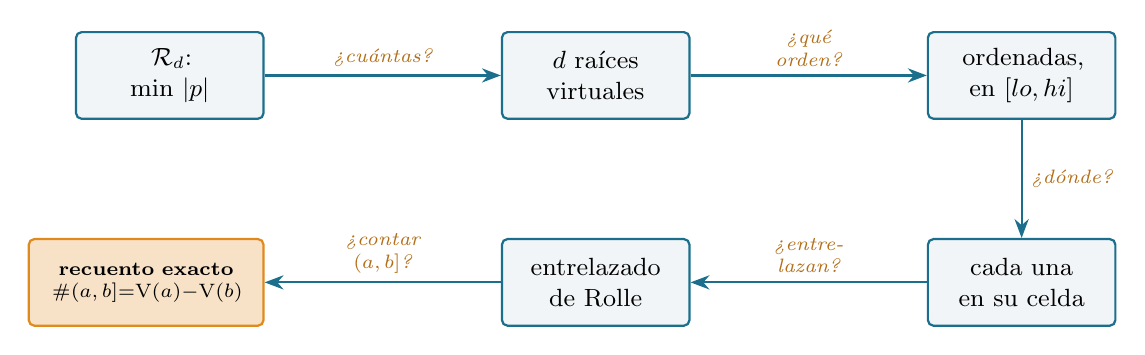
\begin{tikzpicture}[
  obj/.style={draw=ggteal,thick,rounded corners=2pt,fill=ggband!40,align=center,
    font=\small,inner sep=4pt,minimum height=11mm,text width=21mm},
  q/.style={font=\scriptsize\itshape,text=ggamber!80!black,align=center,fill=white,inner sep=1pt},
  arr/.style={-{Stealth[length=2.4mm]},thick,ggteal}]
  \node[obj] (op) {$\Rd_d$:\\min $|p|$};
  \node[obj,right=30mm of op] (build) {$d$ ra\'ices\\virtuales};
  \node[obj,right=30mm of build] (order) {ordenadas,\\en $[lo,hi]$};
  \node[obj,below=15mm of order] (loc) {cada una\\en su celda};
  \node[obj,left=30mm of loc] (inter) {entrelazado\\de Rolle};
  \node[obj,left=30mm of inter,fill=ggamber!25,draw=ggamber,font=\scriptsize,text width=27mm] (count)
    {\textbf{recuento exacto}\\$\#(a,b]{=}\V(a){-}\V(b)$};
  \draw[arr] (op) -- node[q,above=2pt] {¿cu\'antas?} (build);
  \draw[arr] (build) -- node[q,above=2pt] {¿qu\'e\\orden?} (order);
  \draw[arr] (order) -- node[q,right=2pt,fill=none] {¿d\'onde?} (loc);
  \draw[arr] (loc) -- node[q,above=2pt] {¿entre-\\lazan?} (inter);
  \draw[arr] (inter) -- node[q,above=2pt] {¿contar\\$(a,b]$?} (count);
\end{tikzpicture}
\caption{El mapa del lector. Del operador de elecci\'on $\Rd_d$ a un recuento certificado en un
intervalo; cada flecha es la pregunta que responde su secci\'on, y cada nodo es un bloque de Lean
\lean{sorry}-free. La cadena limpia---operador, $d$ ra\'ices, orden, localizaci\'on por celda,
entrelazado, recuento---es la arquitectura sobre la que se sostiene todo el desarrollo.}
\label{fig:readermap}
\end{figure}

\section{Un recuento que no tiembla}\label{sec:intro}

¿Cu\'antas ra\'ices tiene un polinomio? La respuesta honesta tiembla. Un polinomio real de grado $d$
tiene \emph{entre $0$ y $d$} ra\'ices reales, y el n\'umero da bandazos al mover los coeficientes:
$x^2-t$ tiene dos ra\'ices reales, luego una, luego ninguna a medida que $t$ cae por debajo de cero,
mientras su grado nunca cambia. Un recuento que salta cuando nada esencial lo ha hecho es un mal
recuento. \textbf{Hay uno mejor: un polinomio de grado $d$ tiene siempre exactamente $d$ \emph{ra\'ices
virtuales}}---n\'umeros reales $\rho_{d,1}(p)\le\cdots\le\rho_{d,d}(p)$ que coinciden con las ra\'ices
genuinas cuando existen y, si no, se sit\'uan donde el polinomio m\'as se acerca a anularse. No saltan,
no desaparecen y var\'ian de forma continua con los coeficientes. Este paper verifica por m\'aquina la
teor\'ia estructural de ese recuento mejor.

La imagen que conviene retener es la m\'as simple no trivial. El polinomio $p=x^2+1$ no tiene ra\'iz
real, pero su gr\'afica baja a un \'unico acercamiento m\'aximo en $x=0$. Las ra\'ices virtuales ven
ese acercamiento: $p$ tiene la ra\'iz virtual doble $\rho_{2,1}=\rho_{2,2}=0$
(Figura~\ref{fig:fillin}). Donde habr\'ia una ra\'iz real, hay una virtual; donde se esconden dos
ra\'ices conjugadas, las dos ra\'ices virtuales colisionan en el fondo de la hondonada en vez de
desaparecer. Nada se inventa---la construcci\'on es expl\'icita y semialgebraica---y nada se pierde:
\textbf{el recuento siempre es $d$}. El hilo conductor del paper es ese contraste: las ra\'ices reales
son un recuento que tiembla y las virtuales son la familia estable de $d$ elementos por debajo, y la
estabilidad no se afirma sino que se \emph{construye}, lo bastante concreta como para que un n\'ucleo
la verifique.

La pregunta es vieja, y tambi\'en sus respuestas. Descartes (1637) acot\'o las ra\'ices positivas por
los cambios de signo de los coeficientes; Budan y Fourier (1807--1831) leyeron el mismo recuento en la
torre de derivadas $p,p',p'',\dots$; Sturm (1835) lo hizo exacto, pero solo para ra\'ices
\emph{distintas}. Cada una de estas reglas cuenta una cantidad que tiembla---las ra\'ices reales---as\'i
que las de Budan y Fourier solo la \emph{acotan}, con un excedente par que nadie supo nombrar. El
arreglo lleg\'o tarde: Gonz\'alez-Vega, Lombardi y Mah\'e aislaron las ra\'ices virtuales en
1998~\cite{glm}, la familia estable de $d$ elementos para la que esa cota se vuelve igualdad (Coste,
Lajous, Lombardi y Roy~\cite{coste}). Este paper verifica por m\'aquina esa familia---su construcci\'on,
su recuento, su orden y el entrelazado de Rolle---y luego la igualdad misma
(Secci\'on~\ref{sec:count}): el excedente, resulta, no era m\'as que el recuento mirando las ra\'ices
equivocadas. Llegu\'e a \'el como llegu\'e a Sturm~\cite{sturmlean} y a Budan--Fourier~\cite{bflean}:
preguntando qu\'e resultados cl\'asicos de recuento de ra\'ices le faltan a una biblioteca madura, y
hallando las ra\'ices virtuales ausentes de todo asistente que pude buscar.

\begin{figure}[htbp]
\centering
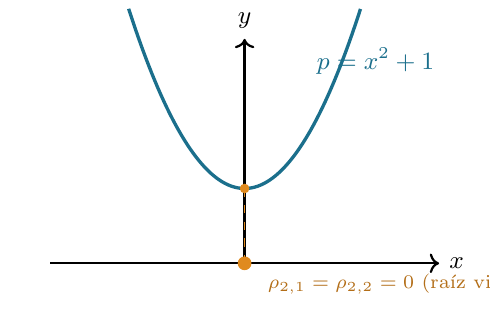
\begin{tikzpicture}[scale=0.95]
  \useasboundingbox (-2.9,-0.6) rectangle (2.9,3.15);
  \draw[->,thick] (-2.6,0) -- (2.6,0) node[right,font=\small] {$x$};
  \draw[->,thick] (0,0) -- (0,3.0) node[above,font=\small] {$y$};
  \draw[ggteal,very thick,domain=-1.55:1.55,samples=80] plot (\x,{\x*\x+1});
  \node[ggteal,font=\small] at (1.75,2.7) {$p=x^2+1$};
  \filldraw[ggamber] (0,1) circle (1.6pt);
  \draw[ggamber,dashed] (0,1) -- (0,0);
  \filldraw[ggamber] (0,0) circle (2.4pt);
  \node[ggamber!80!black,font=\scriptsize,anchor=west] at (0.18,-0.28)
    {$\rho_{2,1}=\rho_{2,2}=0$ (ra\'iz virtual doble)};
\end{tikzpicture}
\caption{Ra\'ices que siempre est\'an ah\'i. El polinomio $x^2+1$ no tiene ra\'iz real, pero s\'i una
ra\'iz virtual doble en $x=0$, donde la gr\'afica m\'as se acerca al eje. Un polinomio de grado~$2$
tiene dos ra\'ices virtuales sea cual sea su discriminante; aqu\'i coinciden. En Lean, sobre un
intervalo de encuadre, la construcci\'on devuelve la lista \lean{[0,\,0]}.}
\label{fig:fillin}
\end{figure}

\section{Las \texorpdfstring{$d$}{d} ra\'ices que siempre est\'an ah\'i}\label{sec:q1}

La idea de que un polinomio carga $d$ ``ra\'ices'' reales can\'onicas con independencia de cu\'antas
sean genuinas es de Gonz\'alez-Vega--Lombardi--Mah\'e~\cite{glm}, enmarcada en la teor\'ia de
variaci\'on de signos cuyo tratamiento de libro es Basu--Pollack--Roy~\cite{bpr}, Cap.~2. La
definici\'on es \lean{vroots} y el recuento es \lean{vroots\_length}.

Entre dos puntos cr\'iticos consecutivos de $p$---dos ra\'ices
consecutivas de $p'$---la derivada mantiene signo constante, as\'i que $p$ es estrictamente
mon\'otona ah\'i y $|p|$ tiene un \'unico m\'inimo. El punto donde se alcanza ese m\'inimo es una
ra\'iz virtual: la \'unica ra\'iz de $p$ en la celda si $p$ cambia de signo a trav\'es de ella, y si
no, el extremo de la celda donde $p$ es menor. Los puntos cr\'iticos de $p$ son las ra\'ices virtuales
de $p'$, as\'i que la construcci\'on recurre en la derivada, igual que el teorema de Rolle~\cite{rolle}
intercala las ra\'ices de $p$ y $p'$.

\emph{Por qu\'e exactamente $d$.} Un polinomio de grado $d$ tiene una derivada de grado $d-1$,
luego---por inducci\'on---$d-1$ ra\'ices virtuales de $p'$; estas cortan la recta en $d$ celdas, y
cada celda aporta una ra\'iz virtual de $p$. El recuento nunca degenera: es el grado, no el n\'umero
de ra\'ices reales. Este es el primer teorema, y el m\'as limpio:
\keyeq{\#\,\{\text{ra\'ices virtuales de }p\} \;=\; \deg p .}
En Lean es \lean{vroots\_length}: la lista \lean{vroots lo hi p} de ra\'ices virtuales tiene longitud
\lean{p.natDegree}. Las ra\'ices reales son a lo sumo $d$ (y pueden ser muchas menos, o ninguna);
\textbf{las virtuales son siempre exactamente $d$}. La diferencia entre ambos recuentos es precisamente
el excedente par de Budan--Fourier, ahora realizado como colisiones de ra\'ices virtuales fuera del
eje.

La receta es limpia sobre el papel---\emph{minimiza $|p|$ en cada celda $p'$-mon\'otona}---pero ``el
punto donde $|p|$ es menor'' es una elecci\'on, y ``las celdas'' las corta un objeto definido por la
misma recursi\'on. Ambas han de hacerse expl\'icitas antes de que un n\'ucleo las acepte.

\section{Constru\'irlas: el operador de elecci\'on \texorpdfstring{$\Rd_d$}{R\_d}}\label{sec:q2}

La construcci\'on recursiva---cortar la recta por los puntos cr\'iticos, minimizar $|p|$ en cada
trozo---es la definici\'on de Gonz\'alez-Vega--Lombardi--Mah\'e~\cite{glm}, ligada al recuento de
variaci\'on de signos por Coste~\cite{coste}. Donde una prueba a mano dice ``toma el punto donde $|p|$
es menor'', una formal debe producirlo: ese es el operador \lean{R} (existencia
\lean{exists\_isMinOn\_abs\_eval}), ensamblado por la recursi\'on \lean{vroots}.

Las celdas de $p$ las cortan las ra\'ices virtuales de $p'$ junto con
dos vallas exteriores. En vez de trabajar en todo $\R$ desde el principio, fijo un intervalo cerrado
$[lo,hi]$ y construyo las ra\'ices virtuales dentro de \'el; tomar $lo,hi$ m\'as all\'a de toda ra\'iz
de la torre de derivadas (una cota de Cauchy) recupera el objeto global, y ese \'ultimo paso se
comenta en la Secci\'on~\ref{sec:boundary}. Trabajar en $[lo,hi]$ mantiene toda cantidad como n\'umero
real genuino y deja a la recursi\'on reutilizar un \'unico operador de elecci\'on.

\emph{El operador de elecci\'on $\Rd_d$.} En un intervalo cerrado $[a,b]$, la funci\'on continua
$|p|$ alcanza un m\'inimo (el intervalo es compacto); llamamos $\Rd_d(a,b,p)$ a un minimizador. En
Lean es \lean{R}, definido eligiendo un minimizador cuya existencia es \lean{exists\_isMinOn\_abs\_eval}.
Dos hechos sobre \'el cargan toda la teor\'ia. Primero, \textbf{cae en el intervalo}: \lean{R\_mem}
dice $\Rd_d(a,b,p)\in[a,b]$. Segundo, \textbf{capta las ra\'ices reales}: si $p(a)\le 0\le p(b)$ (o al
rev\'es), el teorema del valor intermedio da una ra\'iz, el m\'inimo de $|p|$ es entonces $0$, y el
minimizador es esa ra\'iz---\lean{R\_eval\_eq\_zero\_of\_le\_zero\_le}. As\'i que en una celda donde
$p$ cambia de signo, $\Rd_d$ es la ra\'iz genuina; donde no, es el extremo m\'as cercano. Ese es el
sentido preciso en que las ra\'ices virtuales extienden a las reales.

\begin{recipebox}{El operador de elecci\'on $\Rd_d(a,b,p)$ (receta)}
En un intervalo cerrado $[a,b]$, toma \textbf{cualquier minimizador de $|p|$} (existe, $[a,b]$ es
compacto). Dos hechos bastan para toda la teor\'ia. \textbf{Cae en el intervalo},
$\Rd_d(a,b,p)\in[a,b]$ (\lean{R\_mem}); este \'unico hecho da el entrelazado. \textbf{Es una ra\'iz
real cuando $p$ tiene una}: si $p$ cambia de signo en $[a,b]$, el m\'inimo de $|p|$ es $0$, luego
$\Rd_d$ es una ra\'iz genuina (\lean{R\_eval\_eq\_zero\_of\_le\_zero\_le}); as\'i extienden las
virtuales a las reales. La unicidad, donde $p'$ mantiene signo, sale gratis de los ladrillos de
monoton\'ia de la secci\'on siguiente---as\'i que el minimizador \emph{elegido} es de hecho el \'unico.
\end{recipebox}

\emph{La recursi\'on.} Las ra\'ices virtuales se ensamblan listando los breakpoints
\[
  \mathrm{bps} \;=\; lo \,::\, \big(\text{ra\'ices virtuales de }p'\big) \,+\!\!+\, [\,hi\,],
\]
y aplicando $\Rd_d$ a cada par consecutivo:
$\lean{vroots}\,lo\,hi\,p = \lean{zipWith}\;(\Rd_d\,p)\;\mathrm{bps}\;\mathrm{bps.tail}$. Un polinomio
de grado~$0$ no tiene ra\'ices virtuales; en otro caso la recursi\'on desciende a $p'$, terminando
porque $\deg p' < \deg p$ (\lean{natDegree\_derivative\_lt}). La definici\'on bien fundada y el teorema
de longitud son el contenido de \lean{vroots} y \lean{vroots\_length} (Figura~\ref{fig:construct}).

\begin{figure}[htbp]
\centering
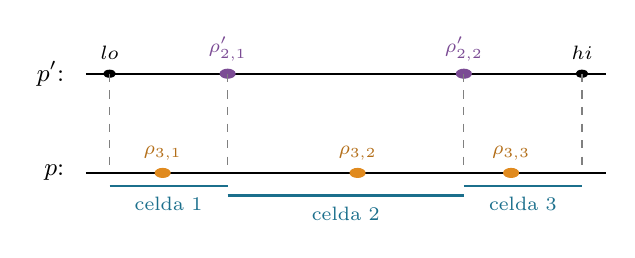
\begin{tikzpicture}[xscale=1.5,yscale=0.9]
  \draw[thick] (-2.2,1.4) -- (2.2,1.4);
  \node[left,font=\small] at (-2.3,1.4) {$p'$:};
  \foreach \x in {-1,1} \filldraw[ggplum] (\x,1.4) circle (1.8pt);
  \node[ggplum,font=\scriptsize,above=1pt] at (-1,1.4) {$\rho'_{2,1}$};
  \node[ggplum,font=\scriptsize,above=1pt] at (1,1.4) {$\rho'_{2,2}$};
  \node[font=\scriptsize] at (-2,1.7) {$lo$};
  \node[font=\scriptsize] at (2,1.7) {$hi$};
  \filldraw (-2,1.4) circle (1.4pt); \filldraw (2,1.4) circle (1.4pt);
  \draw[thick] (-2.2,0) -- (2.2,0);
  \node[left,font=\small] at (-2.3,0) {$p$:};
  \foreach \x in {-2,-1,1,2} \draw[gray,dashed] (\x,1.4) -- (\x,0);
  \draw[ggteal,thick] (-2,-0.18) -- (-1,-0.18); \node[ggteal,font=\scriptsize,below] at (-1.5,-0.2) {celda 1};
  \draw[ggteal,thick] (-1,-0.32) -- (1,-0.32);  \node[ggteal,font=\scriptsize,below] at (0,-0.34) {celda 2};
  \draw[ggteal,thick] (1,-0.18) -- (2,-0.18);   \node[ggteal,font=\scriptsize,below] at (1.5,-0.2) {celda 3};
  \foreach \x in {-1.55,0.1,1.4} \filldraw[ggamber] (\x,0) circle (1.8pt);
  \node[ggamber!80!black,font=\scriptsize,above=1pt] at (-1.55,0) {$\rho_{3,1}$};
  \node[ggamber!80!black,font=\scriptsize,above=1pt] at (0.1,0) {$\rho_{3,2}$};
  \node[ggamber!80!black,font=\scriptsize,above=1pt] at (1.4,0) {$\rho_{3,3}$};
\end{tikzpicture}
\caption{La recursi\'on, para $\deg p = 3$. Las dos ra\'ices virtuales de $p'$ (ciruela) junto con las
vallas $lo,hi$ cortan $[lo,hi]$ en tres celdas; en cada celda $p'$ mantiene signo constante, as\'i que
$\Rd_d$ devuelve una ra\'iz virtual de $p$ (\'ambar). Cada $\rho_{3,j}$ cae en su propia celda---esto
es lo que las hace salir ordenadas y entrelazadas con las $\rho'_{2,j}$.}
\label{fig:construct}
\end{figure}

\section{Hacer formal la construcci\'on}\label{sec:q3}

La construcci\'on es cl\'asica y el entrelazado tiene una prueba a mano de una l\'inea---``$\Rd_d$ cae
en su celda, y las celdas comparten extremos''---as\'i que lo que cuesta el trabajo no es matem\'atica
nueva sino la contabilidad que hace que una familia recursiva y definida por elecci\'on pase un
n\'ucleo, el an\'alogo de la cirug\'ia de listas que necesit\'o el desarrollo compa\~nero de
Budan--Fourier~\cite{bflean}. Entra en \lean{vroots\_chain\_mem} (el invariante maestro) y
\lean{isChain\_zipWith\_R}.

\emph{Una elecci\'on no computable, usada con honestidad.} $\Rd_d$ es un minimizador \emph{elegido},
as\'i que \lean{R} es \lean{noncomputable} y el desarrollo se apoya en \lean{Classical.choice}. Es
v\'alido y est\'andar, pero significa que las ra\'ices virtuales est\'an especificadas, no calculadas:
los teoremas son sobre \emph{un} minimizador, y lo que los hace inequ\'ivocos es la monoton\'ia. Los
dos \emph{ladrillos de monoton\'ia} compartidos con el trabajo compa\~nero de
Budan--Fourier---\lean{eval\_strictMonoOn\_of\_derivative\_pos} y su gemelo negativo---dicen que donde
$p'$ mantiene signo constante no nulo, $p$ es estrictamente mon\'otona, as\'i que $|p|$ tiene un
\emph{\'unico} pozo y el minimizador es \'unico. El desarrollo formal solo necesita la existencia y los
dos hechos \lean{R\_mem} / \lean{R\_eval\_eq\_zero}; la unicidad es lo que licencia la imagen informal.

\emph{Los breakpoints forman una cadena, y ese es el quid.} Todo lo de aguas abajo descansa en un
invariante: la lista aumentada de breakpoints $lo::(\lean{vroots}\,lo\,hi\,p'\,)+\!\!+[hi]$ est\'a
\emph{ordenada}, y toda ra\'iz virtual cae en $[lo,hi]$. Las dos mitades son mutuamente
dependientes---una lista est\'a ordenada solo si sus miembros est\'an en rango, y $\Rd_d$ cae en rango
solo entre breakpoints ordenados---as\'i que se prueban juntas, por una \'unica inducci\'on que baja la
torre de derivadas (\lean{vroots\_chain\_mem}). El orden es el motor: como
$\Rd_d(\mathrm{bps}[r],\mathrm{bps}[r+1])$ cae en $[\mathrm{bps}[r],\mathrm{bps}[r+1]]$ y los
breakpoints consecutivos est\'an ordenados, las ra\'ices virtuales consecutivas tambi\'en lo est\'an
(\lean{isChain\_zipWith\_R}). Es el teorema de Rolle en forma de lista, y es la parte que la m\'aquina
no me dej\'o esquivar.

\emph{Indexar, y las trampas peque\~nas.} Convertir ``cada ra\'iz virtual cae entre sus breakpoints''
en un enunciado sobre \lean{getElem} exigi\'o un cuidado que una prueba a mano oculta. Reescribir un
acceso indexado que carga prueba (\lean{l[r]} arrastra una prueba $r<\lean{l.length}$) no es un
\lean{rw} sin m\'as; pasa por \lean{simp} con los lemas de \'indice, apoy\'andose en la irrelevancia de
pruebas para conciliar las cotas. Y un \lean{rcases} destructivo sobre una ecuaci\'on $w=lo$
\emph{sustituye} $lo$ en silencio en esa rama---un arreglo de un car\'acter (\lean{le\_rfl} en vez de
\lean{le\_refl lo}), pero del tipo que solo un n\'ucleo detecta. No son profundas, pero son justo los
gestos de la mano que un asistente de pruebas rechaza.

La cadena y la localizaci\'on por \'indice, una vez probadas, son exactamente sobre lo que descansa el
entrelazado.

\section{El entrelazado de Rolle}\label{sec:q4}

Que las ra\'ices de $p$ y $p'$ se intercalen es de Rolle, de 1690~\cite{rolle}; que las
ra\'ices \emph{virtuales} se intercalen del mismo modo---incluso cuando no hay ra\'ices reales---es el
refinamiento de Gonz\'alez-Vega--Lombardi--Mah\'e~\cite{glm} y el n\'ucleo estructural del teorema de
recuento de Coste~\cite{coste}. Es \lean{vroots\_interlacing}, que descansa en la localizaci\'on por
\'indice \lean{vroots\_getElem\_mem}.

La consecuencia principal es el entrelazado de las ra\'ices virtuales
de $p$ con las de $p'$:
\begin{theorem}[Entrelazado de Rolle de ra\'ices virtuales; \lean{vroots\_interlacing}]\label{thm:interlace}
Para $lo\le hi$ y cada \'indice $r$ en rango,
\[
  \rho_{d,r}(p)\ \le\ \rho_{d-1,r}(p')\ \le\ \rho_{d,r+1}(p),
\]
es decir, \lean{(vroots lo hi p)[r] $\le$ (vroots lo hi (derivative p))[r] $\le$ (vroots lo hi p)[r+1]}.
\end{theorem}
\noindent La prueba son dos aplicaciones de la localizaci\'on \lean{vroots\_getElem\_mem}---cada
ra\'iz virtual de $p$ cae entre dos breakpoints---junto con la identidad de que los breakpoints
interiores \emph{son} las ra\'ices virtuales de $p'$. Es la sombra discreta del teorema de Rolle, y
sit\'ua a la familia de ra\'ices virtuales en el mismo plano que las familias entrelazadas que
recorren la literatura de real-rootedness---las desigualdades de Newton, el polinomio de matching de
Heilmann--Lieb---donde una sucesi\'on y su derivada se intercalan. Que esto valga ahora para una
familia definida incluso cuando no hay ra\'ices reales es el punto.

\emph{De qu\'e es el camino.} El entrelazado es la mitad estructural de la historia de Budan--Fourier.
La mitad aritm\'etica---que el n\'umero de ra\'ices virtuales en un intervalo semiabierto $(a,b]$
iguala la ca\'ida de variaciones de signo $\V(a)-\V(b)$ de la torre de derivadas~\cite{coste}---es la
igualdad que la desigualdad cl\'asica de Budan--Fourier~\cite{bflean} solo acota. Funde esta
construcci\'on con una segunda, recursiva de forma independiente, y por eso era la secuela; es el
objeto de la secci\'on siguiente, ya probada.

\section{El recuento exacto}\label{sec:count}

El entrelazado era, en la primera versi\'on de este trabajo, donde el paper se deten\'ia: la teor\'ia
estructural estaba probada y el recuento aritm\'etico se nombraba con honestidad como la secuela. Ya
est\'a probado, y esta secci\'on lo reporta. Es la igualdad para la que era toda la construcci\'on.

\begin{theorem}[El recuento exacto de Budan--Fourier; \lean{card\_vroots\_Ioc\_eq\_fourierVar}]\label{thm:count}
Sup\'ongase que toda ra\'iz de todo miembro de la torre de derivadas $p,p',p'',\dots$ cae estrictamente
dentro de $[lo,hi]$. Entonces para $a\le b$ en $[lo,hi)$,
\[
  \#\{\,\rho\ \text{ra\'iz virtual de }p\ :\ a<\rho\le b\,\}\;=\;\V(a)-\V(b),
\]
donde $\V=\lean{fourierVar}$ es el recuento de variaciones de signo de Budan--Fourier de la torre en un
punto.
\end{theorem}

\noindent En Lean el enunciado es, verbatim (los binders de tipo impl\'icitos $\{lo\,hi:\R\}$,
$\{p:\R[X]\}$ omitidos):
\begin{quote}\ttfamily\small\noindent
theorem card\_vroots\_Ioc\_eq\_fourierVar (hp : p $\neq$ 0)\\
\hspace*{1em}(hbr : Brackets lo hi p) (ha : a $\in$ Ico lo hi) (hb : b $\in$ Ico lo hi) (hab : a $\le$ b) :\\
\hspace*{1em}((vroots lo hi p : Multiset $\mathbb{R}$).filter (fun r => a < r $\wedge$ r $\le$ b)).card\\
\hspace*{2em}= fourierVar p a - fourierVar p b
\end{quote}

\noindent El teorema cl\'asico de Budan--Fourier~\cite{bflean} acota el n\'umero de ra\'ices
\emph{reales} en $(a,b]$ por $\V(a)-\V(b)$, con un excedente par. Reemplaza las ra\'ices reales por las
virtuales y la desigualdad se vuelve igualdad---el excedente nunca fue un defecto del recuento, solo de
\emph{cu\'ales} ra\'ices se contaban. El recuento tembloroso de la Secci\'on~\ref{sec:intro} es lo que
hac\'ia de Budan--Fourier una desigualdad; el recuento estable lo vuelve exacto
(Figura~\ref{fig:staircase}).

\begin{figure}[t]
\centering
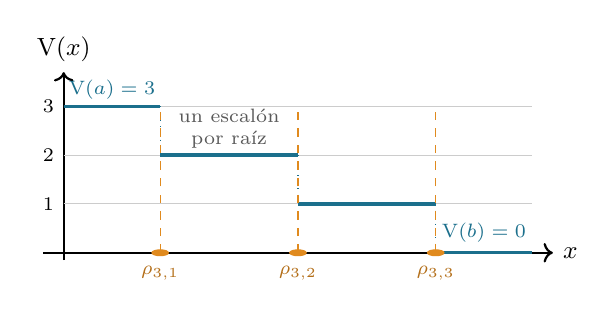
\begin{tikzpicture}[xscale=1.75,yscale=0.62]
  \draw[->,thick] (-1.85,0) -- (1.85,0) node[right,font=\small] {$x$};
  \draw[->,thick] (-1.7,-0.15) -- (-1.7,3.7) node[above,font=\small] {$\V(x)$};
  \foreach \y in {1,2,3} {\node[font=\scriptsize,left] at (-1.7,\y) {$\y$}; \draw[black!20] (-1.7,\y)--(1.7,\y);}
  \draw[ggteal,very thick] (-1.7,3) -- (-1,3);
  \draw[ggteal,very thick] (-1,2) -- (0,2);
  \draw[ggteal,very thick] (0,1) -- (1,1);
  \draw[ggteal,very thick] (1,0) -- (1.7,0);
  \draw[ggteal,dotted] (-1,3)--(-1,2); \draw[ggteal,dotted] (0,2)--(0,1); \draw[ggteal,dotted] (1,1)--(1,0);
  \foreach \x in {-1,0,1} {\draw[ggamber,dashed] (\x,0)--(\x,{3+\x*0});}
  \foreach \x in {-1,0,1} \filldraw[ggamber] (\x,0) circle (1.7pt);
  \node[ggamber!80!black,font=\scriptsize,below=1pt] at (-1,-0.02) {$\rho_{3,1}$};
  \node[ggamber!80!black,font=\scriptsize,below=1pt] at (0,-0.02) {$\rho_{3,2}$};
  \node[ggamber!80!black,font=\scriptsize,below=1pt] at (1,-0.02) {$\rho_{3,3}$};
  \node[ggteal,font=\scriptsize] at (-1.35,3.35) {$\V(a)=3$};
  \node[ggteal,font=\scriptsize] at (1.35,0.42) {$\V(b)=0$};
  \node[font=\scriptsize,text=black!65,align=center] at (-0.5,2.55) {un escal\'on\\por ra\'iz};
\end{tikzpicture}
\caption{El recuento exacto como escalera. Para $p=x^3-x$ el recuento de Budan--Fourier $\V(x)$ es plano
entre ra\'ices virtuales y baja exactamente uno en cada una; el n\'umero de ra\'ices virtuales en
$(a,b]$ es el descenso total $\V(a)-\V(b)$. Aqu\'i $\V(a)-\V(b)=3$ para cualquier $a<-1$ y $b>1$,
coincidiendo con las tres ra\'ices virtuales $\rho_{3,1}<\rho_{3,2}<\rho_{3,3}$ (todas reales para este
$p$). Una colisi\'on de grado dos, como en la Figura~\ref{fig:fillin}, aparecer\'ia como un \'unico
escal\'on de altura dos---el recuento sigue exacto, leyendo ahora una ra\'iz virtual que el recuento de
ra\'ices reales no ve.}
\label{fig:staircase}
\end{figure}

\emph{Por qu\'e es un teorema y no una l\'inea.} Funde las dos recursiones de las que est\'a hecho el
desarrollo. Tanto $\V$ como \lean{vroots} bajan la misma torre $p\to p'$---$\V$ pelando el signo
principal, \lean{vroots} por el entrelazado de Rolle---pero son objetos \emph{a priori} distintos, y el
teorema es que marchan al un\'isono. La prueba pasa por la reformulaci\'on
\[
  \V_p(x)\;=\;\#\{\text{ra\'ices virtuales de }p \text{ estrictamente por encima de } x\}
\]
(\lean{fourierVar\_eq\_card\_vroots\_gt}, por inducci\'on que baja la torre), de la que el recuento en
$(a,b]$ sale por resta; el teorema del intervalo es entonces una partici\'on de multiconjunto. El paso
inductivo es un \'unico lema por escal\'on (\lean{count\_step}): de $p'$ a $p$, el recuento de ra\'ices
virtuales por encima de $x$ sube exactamente el incremento de Fourier $\V_p(x)-\V_{p'}(x)$, y ese
incremento es $0$ o $1$.

\emph{D\'onde se encuentran los dos bits.} Localiza $x$ en su celda $[\mathrm{bps}[i],\mathrm{bps}[i+1]]$
de la partici\'on de breakpoints de $p'$ (Figura~\ref{fig:construct}). El entrelazado ya obliga a cada
celda estrictamente por encima de $x$ a aportar una ra\'iz virtual de $p$ y a cada celda por debajo a no
aportar ninguna, as\'i que todo el incremento es si la \'unica ra\'iz virtual $v_i$ \emph{en la propia
celda de $x$} cae por encima de $x$ (\lean{count\_diff\_eq\_cell}). En esa celda $p'$ no tiene ra\'iz---una
ra\'iz de $p'$ ser\'ia una ra\'iz virtual de $p'$, es decir un breakpoint, y ninguno cae estrictamente
entre dos breakpoints consecutivos (Prop.~2.2 de Coste, aqu\'i \lean{root\_mem\_vroots})---as\'i que $p$
es estrictamente mon\'otona a trav\'es de ella, y su minimizador de $|p|$, $v_i$, cae por encima de $x$
exactamente cuando $p(x)$ tiene el signo que a\'un no ha ``doblado la esquina'' hacia la ra\'iz
(\lean{lt\_R\_iff\_eval\_neg} y su gemelo).

\emph{El \'unico paso anal\'itico.} En el lado de Fourier el incremento es $1$ exactamente cuando
$\mathrm{sign}\,p(x)$ discrepa del primer signo superviviente $d$ de la torre $p',p'',\dots$ en $x$. El
puente entre los dos lados es una identidad:
\keyeq{d \;=\; \text{el signo de } p' \text{ en la celda de } x.}
La derivada de orden m\'as bajo que no se anula en $x$ fija $p'$ justo a la derecha de $x$, y en la
celda sin ra\'ices ese signo es constante; as\'i que $d$ es la direcci\'on de monoton\'ia de la celda.
(En Lean es \lean{fourier\_head\_right}, reutilizando \lean{signs\_right\_eq\_Rseq} del trabajo
compa\~nero~\cite{bflean}: el patr\'on de signos justo a la derecha de $x$ es el patr\'on superviviente
principal en $x$.) Esta identidad es la que elimina la contabilidad de multiplicidades que vuelve
delicada la prueba cl\'asica: una vez fijado $d$ a la celda, ``$v_i$ por encima de $x$'' y ``una nueva
variaci\'on de Fourier'' son el \emph{mismo} suceso, y las dos recursiones coinciden t\'ermino a
t\'ermino. Sumar los escalones da el Teorema~\ref{thm:count} (Figura~\ref{fig:staircase}).

\emph{Qu\'e necesita y qu\'e no.} La hip\'otesis de encuadre---toda ra\'iz de la torre estrictamente
dentro de $[lo,hi]$---es justo lo que hace limpio el recuento: $\V(lo)$ es el grado, $\V(hi)=0$, y toda
ra\'iz virtual es interior. Es la misma disciplina de intervalo fijo que la construcci\'on
(Secci\'on~\ref{sec:q2}); levantarla a todo $\R$ por una cota de Cauchy es el mismo paso diferido
(Secci\'on~\ref{sec:boundary}). No se calcula ninguna ra\'iz ni se construye ning\'un aislador---el
teorema certifica el recuento, no un procedimiento.

\section{Qu\'e habilita una teor\'ia certificada de ra\'ices virtuales}\label{sec:enables}

Una familia de ra\'ices virtuales verificada por m\'aquina es el t\'ermino medio que falta entre dos
cosas que Mathlib ya tiene y una que no ten\'ia. Tiene la regla de Descartes (el recuento de signos de
coeficientes) y, en el trabajo compa\~nero, la \emph{desigualdad} de Budan--Fourier; no ten\'ia el
objeto que vuelve esa desigualdad una igualdad. Las ra\'ices virtuales son ese objeto, y la
Secci\'on~\ref{sec:count} cierra la igualdad. Aguas abajo, son la entrada correcta para un
procedimiento certificado de \emph{aislamiento} de ra\'ices reales en la l\'inea de Vincent, Collins y
Akritas~\cite{vincent,collinsakritas,akritas} y la teor\'ia de variaci\'on de signos de
Basu--Pollack--Roy~\cite{bpr}---el recuento es ahora exacto, as\'i que un m\'etodo de subdivisi\'on que
lee $\V(a)-\V(b)$ en cada mitad tiene, en principio, una garant\'ia verificada sobre la que construir. Y como la familia
est\'a definida para todo polinomio, con ra\'ices reales o sin ellas, conecta los m\'etodos de
intervalo con el \'algebra del discriminante: un par de ra\'ices virtuales colisiona exactamente cuando
dos ra\'ices reales est\'an a punto de volverse complejas, que es de donde sale el excedente par de
Budan--Fourier (Figura~\ref{fig:bifurc}). La teor\'ia estructural formalizada aqu\'i es el cimiento
sobre el que se sostiene todo eso.

\begin{figure}[H]
\centering
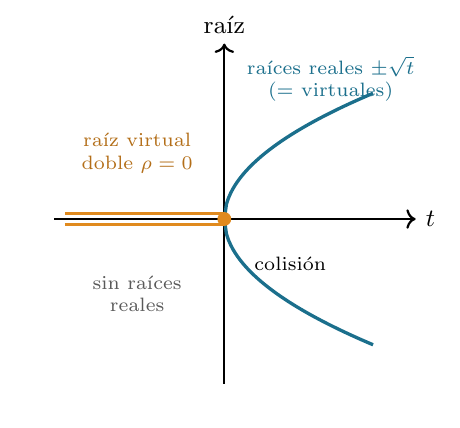
\begin{tikzpicture}[scale=1.35]
  \useasboundingbox (-1.85,-1.7) rectangle (1.95,1.8);
  \draw[->,thick] (-1.6,0) -- (1.8,0) node[right,font=\small] {$t$};
  \draw[->,thick] (0,-1.55) -- (0,1.65) node[above,font=\small] {ra\'iz};
  \draw[ggteal,very thick,domain=0:1.4,samples=70] plot ({\x},{sqrt(\x)});
  \draw[ggteal,very thick,domain=0:1.4,samples=70] plot ({\x},{-sqrt(\x)});
  \draw[ggamber,very thick] (-1.5,0.05) -- (0,0.05);
  \draw[ggamber,very thick] (-1.5,-0.05) -- (0,-0.05);
  \filldraw[ggamber] (0,0) circle (1.7pt);
  \node[ggteal,font=\scriptsize,align=center] at (1.0,1.32) {ra\'ices reales $\pm\sqrt{t}$\\($=$ virtuales)};
  \node[ggamber!80!black,font=\scriptsize,align=center] at (-0.82,0.62) {ra\'iz virtual\\doble $\rho=0$};
  \node[font=\scriptsize,align=center,text=black!65] at (-0.82,-0.7) {sin ra\'ices\\reales};
  \node[font=\scriptsize] at (0.62,-0.42) {colisi\'on};
\end{tikzpicture}
\caption{Ra\'ices que siempre est\'an ah\'i, al mover un par\'ametro. Para $p_t=x^2-t$ las dos ra\'ices
reales $\pm\sqrt{t}$ (teal) existen solo para $t\ge 0$ y desaparecen al caer $t$ por debajo de $0$; las
dos ra\'ices \emph{virtuales} (\'ambar) persisten para \emph{todo} $t$, coincidiendo con las reales
cuando $t\ge 0$ y colisionando en la ra\'iz virtual doble $\rho=0$ para $t<0$. El recuento de ra\'ices
reales salta $2\to 0$ en $t=0$; el de virtuales se queda en $2$. La colisi\'on en $t=0$ es exactamente
donde se forma un par conjugado---el origen del excedente par de Budan--Fourier. (Otra vista del mismo
fen\'omeno que la Figura~\ref{fig:fillin}, ahora en movimiento.)}
\label{fig:bifurc}
\end{figure}

\section{Las piezas}\label{sec:blocks}

La Tabla~\ref{tab:results} re\'une los resultados que soportan el peso, todos \lean{sorry}-free en
\lean{VirtualRoots.lean}; la Tabla~\ref{tab:metrics} mide el desarrollo. La dependencia es corta: los
ladrillos de monoton\'ia dan la existencia y las dos propiedades de $\Rd_d$; la inducci\'on combinada
\lean{vroots\_chain\_mem} prueba orden y rango a la vez; y la localizaci\'on por \'indice da el
entrelazado.

\begin{table}[H]
  \centering\footnotesize
  \arrayrulecolor{ggteal}
  \begin{tabular}{@{}llc@{}}
    \toprule
    \rowcolor{ggteal}
    \textcolor{white}{\textbf{Nombre Lean}} & \textcolor{white}{\textbf{Enunciado}} & \textcolor{white}{\textbf{Estado}} \\
    \midrule
    \rowcolor{ggband}
    \lean{R\_mem} & $\Rd_d(a,b,p)\in[a,b]$ & probado \\
    \lean{R\_eval\_eq\_zero\_of\_le\_zero\_le} & $p(a)\!\le\!0\!\le\!p(b)\Rightarrow p(\Rd_d(a,b,p))=0$ & probado \\
    \rowcolor{ggband}
    \lean{vroots\_length} & $\#\{\text{ra\'ices virtuales de }p\}=\deg p$ & probado \\
    \lean{vroots\_isChain} & $lo::(\text{vroots }p)+\!\!+[hi]$ ordenada & probado \\
    \rowcolor{ggband}
    \lean{vroots\_subset\_Icc} & toda ra\'iz virtual cae en $[lo,hi]$ & probado \\
    \lean{vroots\_getElem\_mem} & $\mathrm{bps}[r]\le\rho_{d,r}(p)\le\mathrm{bps}[r{+}1]$ & probado \\
    \rowcolor{ggband}
    \lean{vroots\_interlacing} & $\rho_{d,r}(p)\le\rho_{d-1,r}(p')\le\rho_{d,r+1}(p)$ & probado \\
    \midrule
    \lean{fourierVar\_eq\_card\_vroots\_gt} & $\V_p(x)=\#\{\text{ra\'ices virtuales}>x\}$ & probado \\
    \rowcolor{ggband}
    \lean{count\_step} & puente por escal\'on $\V_p{-}\V_{p'}=$ incremento de celda & probado \\
    \lean{card\_vroots\_Ioc\_eq\_fourierVar} & $\#$ en $(a,b]=\V(a)-\V(b)$ & probado \\
    \bottomrule
  \end{tabular}
  \arrayrulecolor{black}
  \caption{La teor\'ia de las ra\'ices virtuales, toda \lean{sorry}-free: los resultados estructurales
  en \lean{VirtualRoots.lean} (arriba) y el recuento exacto en \lean{VirtualRootsCount.lean} (abajo),
  Lean~4 / Mathlib. \lean{\#print axioms} sobre \lean{vroots\_interlacing} y sobre
  \lean{card\_vroots\_Ioc\_eq\_fourierVar} reporta solo \lean{propext}, \lean{Classical.choice},
  \lean{Quot.sound}.}
  \label{tab:results}
\end{table}

\begin{table}[H]
  \centering\footnotesize
  \arrayrulecolor{ggteal}
  \begin{tabular}{@{}lc@{}}
    \toprule
    \rowcolor{ggteal}
    \textcolor{white}{\textbf{Cantidad}} & \textcolor{white}{\textbf{Valor}} \\
    \midrule
    \rowcolor{ggband}
    L\'ineas: \lean{VirtualRoots.lean} $/$ \lean{VirtualRootsCount.lean} & $378\,/\,944$ \\
    Teoremas $+$ defs: estructural $/$ recuento & $16{+}2\,/\,33$ \\
    \rowcolor{ggband}
    M\'odulos de Mathlib usados (ambos ficheros, distintos) & $12$ \\
    \lean{sorry} / \lean{admit} / \lean{native\_decide} & $0$ \\
    Axiomas fuera del n\'ucleo de Lean & $0$ (solo \lean{propext}, \lean{Classical.choice}, \lean{Quot.sound}) \\
    \rowcolor{ggband}
    Compilaci\'on, Mathlib precompilado (\lean{VirtualRoots} $/$ recuento) & ${\approx}\,8\text{s}\,/\,9$\,s \\
    Toolchain & Lean~4 (godsil pin v4.30) sobre Mathlib \\
    \bottomrule
  \end{tabular}
  \arrayrulecolor{black}
  \caption{El desarrollo, medido. Build: \lean{lake env lean VirtualRoots.lean} y
  \lean{VirtualRootsCount.lean}, exit~0; el tiempo de compilaci\'on es para verificar cada fichero
  contra un Mathlib precompilado. La huella es deliberadamente ligera---nada de \'algebra pesada,
  porque la construcci\'on es elemental. Los doce m\'odulos de Mathlib son
  \lean{Analysis.Calculus.Deriv.Polynomial}, \lean{Deriv.MeanValue}, \lean{Topology.Algebra.Polynomial},
  \lean{Topology.Order.Compact}, \lean{Topology.Order.IntermediateValue},
  \lean{Algebra.Polynomial.Derivative}, \lean{Algebra.Polynomial.Roots},
  \lean{Algebra.Polynomial.FieldDivision}, \lean{Data.List.Destutter}, \lean{Data.Sign.Basic},
  \lean{Data.Real.Basic} y \lean{Algebra.Ring.Parity}.}
  \label{tab:metrics}
\end{table}

\section{La frontera de la contribuci\'on}\label{sec:boundary}

\emph{Qu\'e est\'a probado.} La teor\'ia estructural de las ra\'ices virtuales $\Rd_d$, sorry-free:
existencia y recuento ($=\deg p$), que est\'an ordenadas y caen en el intervalo de encuadre, que
$\Rd_d$ devuelve una ra\'iz real donde $p$ cambia de signo, y el entrelazado de Rolle
(\lean{VirtualRoots.lean}); y, construido sobre ello, el recuento exacto de Budan--Fourier
$\#\{(a,b]\}=\V(a)-\V(b)$ (\lean{VirtualRootsCount.lean}, Secci\'on~\ref{sec:count}). Son los resultados
de Gonz\'alez-Vega--Lombardi--Mah\'e~\cite{glm} y Coste~\cite{coste} en sus partes estructural y de
recuento. El recuento se prueba sobre un intervalo de encuadre $[lo,hi]$ que contiene estrictamente
toda ra\'iz de la torre.

\emph{Qu\'e no est\'a probado.} Dos cosas, ambas genuinamente m\'as all\'a de los ficheros presentes.
\emph{La continuidad}: que las ra\'ices virtuales var\'ian de forma continua con los
coeficientes---mitad de por qu\'e las introdujeron Gonz\'alez-Vega--Lombardi--Mah\'e~\cite{glm}---no se
toca (Secci\'on~\ref{sec:questions}). \emph{El objeto global}: la construcci\'on y el recuento son sobre
un intervalo de encuadre fijo $[lo,hi]$; recuperar el objeto en todo $\R$ tomando $lo,hi$ m\'as all\'a
de toda ra\'iz de la torre de derivadas (una cota de Cauchy, disponible en Mathlib como
\lean{Polynomial.cauchyBound}) es rutina pero no se realiza aqu\'i.

\emph{Novedad.} Hasta donde s\'e, ni las ra\'ices virtuales ni el recuento exacto de Budan--Fourier a
trav\'es de ellas se hab\'ian formalizado en ning\'un asistente de pruebas antes. La afirmaci\'on se
apoya en b\'usquedas en junio~2026 de: Mathlib (sin ra\'ices virtuales; tiene Descartes v\'ia
\lean{Polynomial.signVariations}); la biblioteca \lean{mathcomp-real-closed} de Coq (ra\'ices reales y
la codificaci\'on de Thom, no ra\'ices virtuales); el AFP de Isabelle, cuya entrada \lean{Budan\_Fourier}
formaliza la desigualdad con multiplicidad pero no el objeto ra\'iz virtual ni la igualdad; y HOL~Light
(Sturm y Descartes, no ra\'ices virtuales). Hago la afirmaci\'on al nivel del objeto nombrado; no puedo
excluir un desarrollo in\'edito o con otro nombre, y agradecer\'ia una indicaci\'on.

\emph{Autor\'ia.} La matem\'atica es cl\'asica, debida a los autores citados. La formalizaci\'on se
realiz\'o en interacci\'on estrecha con un asistente de IA (Claude, Anthropic): la elecci\'on del
objetivo, la arquitectura general de la prueba, los enunciados y las afirmaciones de alcance y novedad
son m\'ias; el asistente redact\'o e iter\'o buena parte del Lean bajo esa direcci\'on. La divisi\'on
no afecta a la validez---una prueba se acepta solo cuando el n\'ucleo de Lean la type-checkea, cosa que
hace, con el perfil de axiomas reportado arriba---pero se enuncia aqu\'i con claridad por atribuci\'on
cient\'ifica.

\section{Qu\'e queda abierto}\label{sec:questions}

Tres hechos marcan hacia d\'onde apunta el trabajo; el primero ya est\'a resuelto y nombra su propia
pregunta pendiente, los otros dos siguen abiertos.

\begin{enumerate}\itemsep3pt
\item \emph{Dos definiciones, un objeto---desde cu\'al formalizar.} Las ra\'ices virtuales tienen dos
definiciones cl\'asicas: la construcci\'on por el minimizador $\Rd_d$ de
Gonz\'alez-Vega--Lombardi--Mah\'e~\cite{glm}, usada aqu\'i, y los valores donde salta \lean{fourierVar},
la definici\'on de Coste et al.~\cite{coste}. Las dos coinciden, y \emph{esa coincidencia es el teorema
de Coste}---no algo que este paper abra. Lo que este paper hace es formalizar la construcci\'on y
\emph{puentearla} a \lean{fourierVar} para el recuento (Secci\'on~\ref{sec:count}). La definici\'on por
saltos har\'ia el recuento casi por definici\'on pero el entrelazado m\'as dif\'icil; as\'i que lo
genuinamente abierto no es la matem\'atica sino la elecci\'on \emph{en Lean}---¿es m\'as barato, en un
asistente de pruebas, re-derivar la equivalencia de Coste desde el lado de los saltos que el puente
tomado aqu\'i? El entrelazado fue gratis en el lado de la construcci\'on, el recuento lo ser\'ia en el
de los saltos; ninguna definici\'on da ambas a la vez.
\item \emph{La continuidad, la otra mitad de su raz\'on de ser.} Las ra\'ices virtuales var\'ian de
forma \emph{continua} con los coeficientes---de hecho Gonz\'alez-Vega--Lombardi--Mah\'e prueban que las
$\rho_{d,j}$ son funciones semialgebraicas continuas~\cite{glm}, que es la mitad de por qu\'e las
introdujeron. La matem\'atica es suya y est\'a resuelta; lo abierto es solo su formalizaci\'on, no
tocada aqu\'i. Una prueba en Lean tendr\'ia que hacer que $\Rd_d$, un minimizador elegido, dependa de
$p$ con continuidad; los ladrillos de monoton\'ia que fijan el minimizador son el punto de partida
natural, pero el enunciado es genuinamente anal\'itico y va m\'as all\'a de la contabilidad algebraica
de este paper.
\item \emph{Un entrelazado, tres caras.} El entrelazado de Rolle sit\'ua a las ra\'ices virtuales junto
a las familias que recorren la literatura de real-rootedness: las ra\'ices de un polinomio y su derivada
(Rolle cl\'asico~\cite{rolle}), las desigualdades de Newton~\cite{newton} y el polinomio de matching de
Heilmann--Lieb. Las \emph{cadenas de Sturm} abstractas de Eisermann~\cite{eisermann} ya axiomatizan una
de esas estructuras de entrelazado. ¿Hay una \'unica noci\'on Lean de ``familia entrelazada'' que
subsuma todas estas---y d\'onde se sit\'ua dentro de ella la familia de ra\'ices virtuales, definida
incluso cuando no hay ra\'ices reales? Esa es la cuenta que m\'as me gustar\'ia llevarme.
\end{enumerate}

\section*{Reproducir}
\begin{verbatim}
git clone https://github.com/karlesmarin/godsil-gutman-lean
cd godsil-gutman-lean && lake exe cache get
lake build BudanFourier         # el toolkit de variacion de signos importado
lake env lean VirtualRoots.lean       # la teoria estructural
lake env lean VirtualRootsCount.lean  # el recuento exacto
\end{verbatim}
{\sloppy Lean~4 (pin de toolchain godsil \lean{v4.30}) sobre Mathlib. Los teoremas estructurales est\'an en
\lean{VirtualRoots.lean} y el recuento exacto \lean{card\_vroots\_Ioc\_eq\_fourierVar} en
\lean{VirtualRootsCount.lean}; sus soportes son la Tabla~\ref{tab:results}. Ambos ficheros son
\lean{sorry}-free, y \lean{\#print axioms} sobre \lean{vroots\_interlacing} y sobre
\lean{card\_vroots\_Ioc\_eq\_fourierVar} reporta solo \lean{propext}, \lean{Classical.choice},
\lean{Quot.sound}. Los signos de cada figura ($x^2+1$, $x^3-x$, $x^2-t$) se re-derivan en aritm\'etica
exacta antes de dibujarla.\par}

\begin{thebibliography}{99}\small
\bibitem{glm} L.~Gonz\'alez-Vega, H.~Lombardi, L.~Mah\'e, Virtual roots of real polynomials,
\emph{J.~Pure Appl.\ Algebra} \textbf{124} (1998), n\'um.~1--3, 147--166.
\bibitem{coste} M.~Coste, T.~Lajous-Loaeza, H.~Lombardi, M.-F.~Roy, Generalized Budan--Fourier theorem
and virtual roots, \emph{J.~Complexity} \textbf{21} (2005), n\'um.~4, 479--486.
\bibitem{descartes} R.~Descartes, \emph{La G\'eom\'etrie} (1637); la regla de los signos acota el
n\'umero de ra\'ices positivas por el n\'umero de cambios de signo de los coeficientes.
\bibitem{budan} F.~D.~Budan de Boislaurent, \emph{Nouvelle m\'ethode pour la r\'esolution des
\'equations num\'eriques}, Par\'is (1807; 2.\textsuperscript{a} ed.\ 1822).
\bibitem{fourier} J.~Fourier, \emph{Analyse des \'equations d\'etermin\'ees}, Firmin Didot, Par\'is
(p\'ostumo, 1831).
\bibitem{rolle} M.~Rolle, \emph{Trait\'e d'alg\`ebre} (1690); entre dos ra\'ices reales consecutivas de
una funci\'on derivable hay una ra\'iz de su derivada.
\bibitem{sturm} C.~Sturm, M\'emoire sur la r\'esolution des \'equations num\'eriques, \emph{M\'emoires
pr\'esent\'es par divers savants \`a l'Acad\'emie Royale des Sciences} \textbf{6} (1835) 271--318.
\bibitem{akritas} A.~G.~Akritas, Reflections on a pair of theorems by Budan and Fourier, \emph{Mathematics
Magazine} \textbf{55} (1982) 292--298.
\bibitem{collinsakritas} G.~E.~Collins, A.~G.~Akritas, Polynomial real root isolation using Descartes'
rule of signs, en \emph{Proc.\ SYMSAC~'76}, ACM, 1976, 272--275.
\bibitem{vincent} A.~Alesina, M.~Galuzzi, A new proof of Vincent's theorem, \emph{L'Enseignement
Math\'ematique} \textbf{44} (1998) 219--256.
\bibitem{bpr} S.~Basu, R.~Pollack, M.-F.~Roy, \emph{Algorithms in Real Algebraic Geometry}, 2.\textsuperscript{a}
ed., Algorithms and Computation in Mathematics \textbf{10}, Springer, 2006 (teor\'ia de variaci\'on de
signos, Cap.~2, y ra\'ices virtuales).
\bibitem{eisermann} M.~Eisermann, The fundamental theorem of algebra made effective: an elementary
real-algebraic proof via Sturm chains, \emph{Amer.\ Math.\ Monthly} \textbf{119} (2012), n\'um.~9,
715--752 (``cadenas de Sturm'' abstractas y el \'indice de Cauchy).
\bibitem{liBF} W.~Li, L.~C.~Paulson, Counting polynomial roots in Isabelle/HOL: a formal proof of the
Budan--Fourier theorem, en \emph{Proc.\ CPP~2019}, ACM, 2019, 52--64; entrada del Archive of Formal
Proofs ``The Budan--Fourier Theorem'' (W.~Li, 2018),
\url{https://isa-afp.org/entries/Budan_Fourier.html} (formaliza la desigualdad con multiplicidad, no el
objeto ra\'iz virtual).
\bibitem{cohen} C.~Cohen, Construction of real algebraic numbers in Coq, en \emph{Interactive Theorem
Proving (ITP 2012)}, LNCS \textbf{7406}, Springer, 2012, 67--82 (base de \lean{mathcomp-real-closed}:
ra\'ices reales y la codificaci\'on de Thom, no ra\'ices virtuales).
\bibitem{eberl} M.~Eberl, Sturm's Theorem, \emph{Archive of Formal Proofs} (2014),
\url{https://isa-afp.org/entries/Sturm_Sequences.html}.
\bibitem{mathlib} The mathlib Community, The Lean mathematical library, en \emph{Certified Programs and
Proofs (CPP 2020)}, ACM, 2020, 367--381.
\bibitem{lean4} L.~de Moura, S.~Ullrich, The Lean~4 theorem prover and programming language, en
\emph{Automated Deduction (CADE~28)}, LNCS \textbf{12699}, Springer, 2021, 625--635.
\bibitem{bflean} C.~Mar\'in, \emph{Contar con la torre de derivadas: el teorema de Budan--Fourier,
verificado por m\'aquina en Lean~4}, Zenodo, 2026, \texttt{doi:10.5281/zenodo.20736143}
(formalizaci\'on compa\~nera; \lean{BudanFourier.lean}).
\bibitem{sturmlean} C.~Mar\'in, \emph{The Staircase of Signs: Sturm's Root-Counting Theorem,
Machine-Checked in Lean~4}, Zenodo, 2026, \texttt{doi:10.5281/zenodo.20707348}.
\bibitem{newton} C.~Mar\'in, \emph{The Inward Bow of a Real-Rooted Polynomial: Newton's Inequalities,
Machine-Checked in Lean~4}, Zenodo, 2026, \texttt{doi:10.5281/zenodo.20693064}.
\end{thebibliography}

\end{document}
